\documentclass[11pt, a4paper]{article}\usepackage[]{graphicx}\usepackage[]{xcolor}
% maxwidth is the original width if it is less than linewidth
% otherwise use linewidth (to make sure the graphics do not exceed the margin)
\makeatletter
\def\maxwidth{ %
  \ifdim\Gin@nat@width>\linewidth
    \linewidth
  \else
    \Gin@nat@width
  \fi
}
\makeatother

\definecolor{fgcolor}{rgb}{0.345, 0.345, 0.345}
\newcommand{\hlnum}[1]{\textcolor[rgb]{0.686,0.059,0.569}{#1}}%
\newcommand{\hlstr}[1]{\textcolor[rgb]{0.192,0.494,0.8}{#1}}%
\newcommand{\hlcom}[1]{\textcolor[rgb]{0.678,0.584,0.686}{\textit{#1}}}%
\newcommand{\hlopt}[1]{\textcolor[rgb]{0,0,0}{#1}}%
\newcommand{\hlstd}[1]{\textcolor[rgb]{0.345,0.345,0.345}{#1}}%
\newcommand{\hlkwa}[1]{\textcolor[rgb]{0.161,0.373,0.58}{\textbf{#1}}}%
\newcommand{\hlkwb}[1]{\textcolor[rgb]{0.69,0.353,0.396}{#1}}%
\newcommand{\hlkwc}[1]{\textcolor[rgb]{0.333,0.667,0.333}{#1}}%
\newcommand{\hlkwd}[1]{\textcolor[rgb]{0.737,0.353,0.396}{\textbf{#1}}}%
\let\hlipl\hlkwb

\usepackage{framed}
\makeatletter
\newenvironment{kframe}{%
 \def\at@end@of@kframe{}%
 \ifinner\ifhmode%
  \def\at@end@of@kframe{\end{minipage}}%
  \begin{minipage}{\columnwidth}%
 \fi\fi%
 \def\FrameCommand##1{\hskip\@totalleftmargin \hskip-\fboxsep
 \colorbox{shadecolor}{##1}\hskip-\fboxsep
     % There is no \\@totalrightmargin, so:
     \hskip-\linewidth \hskip-\@totalleftmargin \hskip\columnwidth}%
 \MakeFramed {\advance\hsize-\width
   \@totalleftmargin\z@ \linewidth\hsize
   \@setminipage}}%
 {\par\unskip\endMakeFramed%
 \at@end@of@kframe}
\makeatother

\definecolor{shadecolor}{rgb}{.97, .97, .97}
\definecolor{messagecolor}{rgb}{0, 0, 0}
\definecolor{warningcolor}{rgb}{1, 0, 1}
\definecolor{errorcolor}{rgb}{1, 0, 0}
\newenvironment{knitrout}{}{} % an empty environment to be redefined in TeX

\usepackage{alltt}

\usepackage[top=1 in, bottom = 1 in, left = 1 in, right = 1 in ]{geometry}

\usepackage{amsmath, amssymb, amsfonts}
\usepackage{enumerate}

\title{006 Mixed Linear Models : An Example}
\author{Ananda Biswas}
\date{}
\IfFileExists{upquote.sty}{\usepackage{upquote}}{}
\begin{document}

\maketitle

A student studies the \textbf{past questions} set by a certain question setter to learn the standards and get an idea about the \textbf{future questions}. Similarly, a statistician studies \textbf{past data} to learn something about the \textbf{data generating process} and get an idea of the \textbf{future data}. Only those aspects of past data are important that are likely to carry through into the future. \\

Suppose we have many plots and we are sowing different varieties of a crop and we want to study the yield of the different varieties. The study was carried out in numerous villages and the villages bring their own effect. So here our box diagram will be :

\begin{figure}[h]
  \centering
  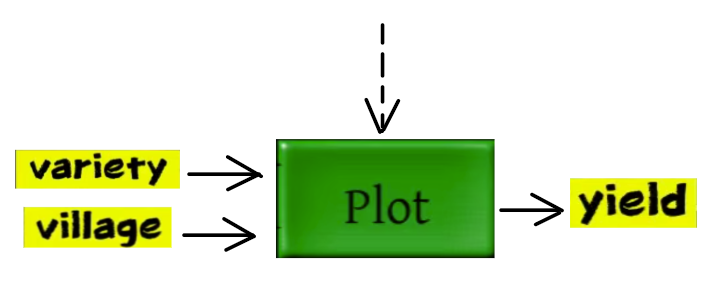
\includegraphics[scale = 0.5]{box_diagram}
\end{figure}

Suppose a \textbf{regular variety} of the crop is currently in use and the government want to introduce a new \textbf{hybrid variety}. Among many villages in West Bengal, 3 villages Chandipur, Barkuti and Mayna were randomly chosen. Here our linear model is ::

$$y_{ijk} = \mu + \alpha_i + \beta_j + \epsilon_{ijk}$$

where $i = 1, 2$, $j = 1, 2, 3$, $k = 1, 2, 3, 4, 5$, $i$ stands for the variety, $j$ stands for the village and $k$ stands for the $kth$ plot for variety $i$ in $jth$ village. \\

Observe that, the 3 villages are just random villages chosen from a population of many villages. We are not at all interested in studying the effect of the villages. So we would like to consider the input village as a random quantity; also called \textbf{random effect}. \\

In our linear model, $j$ is random and $\beta_j$ represents the effect of the $jth$ village. So we shall put another assumption $\beta_j \sim N(0, \sigma_b^2)$. \\

$\beta_j$s are not parameters but random effect. We shall denote it by an English letter. So our linear model is ::

$$y_{ijk} = \mu + \alpha_i + b_j + \epsilon_{ijk}$$

where $i = 1, 2$, $j = 1, 2, 3$, $k = 1, 2, 3, 4, 5$; \\

$\epsilon_{ijk} \sim N(0, \sigma_e^2)$; \\

$b_j \sim N(0, \sigma_b^2)$; \\

$\alpha_i$s are unknown parameters. \\

$b_j$s are random effects and $\alpha_i$s are fixed effects. A linear model which has both random effects and fixed effects is called a \textbf{mixed effects model}. \\


Our linear model can be expressed as :: 

\begin{figure}[h]
  \centering
  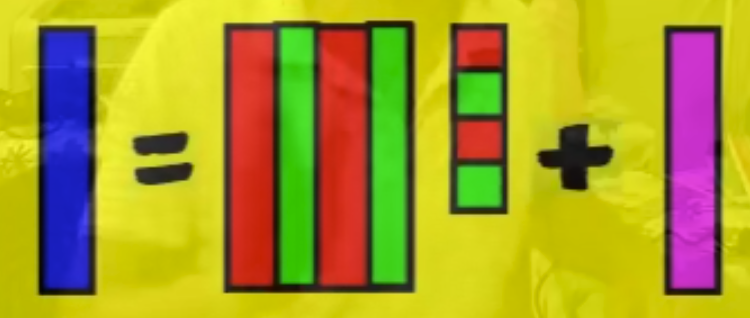
\includegraphics[scale = 0.5]{lm_1}
\end{figure}

The blue vector is the observed values; in the design matrix, the red stripes denote the fixed effects and the green stripes denote the random effects; in the vector of parameters, the red ones are parameters of fixed effects and the green ones are random effects; at last there is a random error vector. \\

The same model can be expressed as ::

\begin{figure}[h]
  \centering
  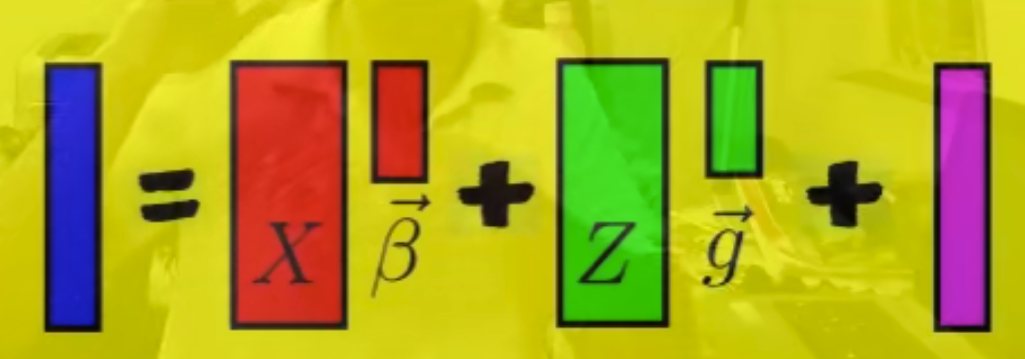
\includegraphics[scale = 0.5]{lm_2}
\end{figure}

Hence ::

$$\vec{y} = X_{n \times p}\vec{\beta} + Z_{n \times q}\vec{g} + \vec{\epsilon}$$

where 

\begin{gather}
	\begin{bmatrix} \vec{g} \\	\vec{\epsilon} \end{bmatrix}
	\sim N_{q+n} \left( \vec{0}, \sigma^2 
	\begin{bmatrix}	G & O \\	O & R	\end{bmatrix} \right)
\end{gather}

or, $\vec{g} \sim N_q \left( \vec{0}, \sigma_e^2I \right)$ and $\vec{\epsilon} \sim N_n \left( \vec{0}, \sigma_b^2I \right)$. \\

$\sigma^2$ is the common scaling factor from $\sigma_e^2I$ and $\sigma_b^2I$. The two null matrices $O$ imply that $\vec{g}$ and $\vec{\epsilon}$ are independent. \\

If we combine the random components and say $\vec{\eta} = Z_{n \times q}\vec{g} + \vec{\epsilon}$, then our linear model can be expressed as ::

$$\vec{y} = X_{n \times p}\vec{\beta} + \vec{\eta}$$

where $\vec{\eta} \sim N_n(\vec{0}, \sigma^2(ZGZ' + R))$.

Observe that, the above is same as a fixed-effects model that we did earlier. Just the interpretation has changed.

\section*{Benefit of Mixed-effects Model : A Real Life Example}

Suppose we want to know what is the real amount of active ingredient that is present in a tablet. We have to do a chemical analysis, and there are various ways to do so. Two such methods of chemical analysis are \textbf{HPLC} and \textbf{NIR}. We want to compare between these two methods. \\

For that, we take lot of similar tablets, split each of them in two parts, allot one part for testing in HPLC method and the other part for testing in NIR method for all the tablets. \\

From HPLC method, we get outputs $y_{1, 1}, y_{1, 2}, \cdots , y_{1, 10}$ and from NIR method we get outputs $y_{2, 1}, y_{2, 2}, \cdots , y_{2, 10}$. \\

One method to compare the two methods HPLC and NIR is \textbf{paired t-test}. We assume $(y_{1, j}, y_{2, j}) \sim $ Bivariate Normal. \\

We shall show that using a linear mixed-effects model can improve upon this test under very similar assumptions. Here our linear model will be :

$$y_{ij} = \mu + \alpha_i + b_j + \epsilon_{ij}$$

where $i = 1, 2$, $j = 1, 2, \cdots, 10$; 

$\alpha_i$s are the parameters of the two different methods; 

$b_j$s are random effects due to the random choice of 10 tablets from a population of tables, ; 

$\epsilon_{ij}$s are random errors. \\

Here we assume $b_j \sim N(0, \tau^2)$ and $\epsilon_{ij} \sim N(0, \sigma^2)$. 

This assumption also captures the fact that $cov(y_{ij}, y_{i'j}) \geq 0$ as they are the readings from two parts of the same tablet. [This additional information could not be captured in the paired t-test.]

\end{document}
